\section{Konzepte (FA)}
Innerhalb dieses Kapitels werden für das Projekt allgemein gültige Strukturen und Aspekte beschrieben, welche bei der Erstellung der Software berücksichtigt werden sollen.

\subsection{Abhängigkeiten zwischen Bausteinen}
Generell sind innerhalb des Projektes folgende Bausteine zu benennen:
\begin{itemize}
	\item Hauptanwendung
	\item Datenbank-API
	\item ExcelReader
	\item baseqt
\end{itemize}
Für den Aufbau der Hauptanwendung wird die Abhängigkeit zu baseqt benötigt. Dadurch ist es möglich sämtliche notwendige Konfigurationen für die Software zu laden und zu initialisieren. Baseqt ermöglicht auch den Aufbau von Dialogen, welche grundsätzliche Informationen über die Anwendung wiedergeben. Allgemein besteht die Hauptanwendung aus einer Ansammlung an Funktionen, jede Funktion ist dabei abhängig von der Datenbank und somit von der Datenbank-API. Dies ist nötig um Daten zu lesen, abzuspeichern oder abzuändern. Die Schülerimport-Funktion benötigt außerdem eine Abhängigkeit zum Excel-Reader. Dieser wird gebraucht, um die Schülerdaten, welche in csv-Dateien abgespeichert werden in interne Datenstrukturen einzulesen und daraufhin in der Datenbank abzuspeichern.

\subsection{Domänenmodell}\label{sec:domaenen}
Innerhalb der Software sollen Schüler und deren Ausleihen und Rückgaben in einer Schulbibliothek dokumentiert werden. Um dies in einer Software abzubilden, benötigt es bestimmte Beziehungen, welche nachfolgend dargestellt werden. Die angegebenen Felder in den Abbildung sind dabei nicht vollständig und dienen hauptsächlich zur Verständnis der Beziehungen untereinander.
\begin{figure}[H]
	\centering
	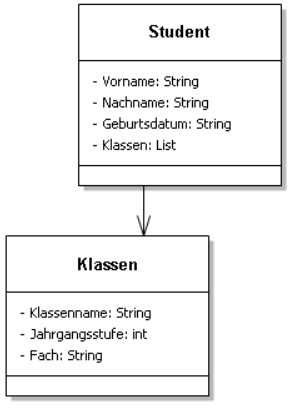
\includegraphics[width=0.30\textwidth]{figures/konzept/studclass.PNG}
	\caption{Beziehung von Schüler und Klasse}
	\label{fig:studclass}
\end{figure}
In Abbildung \ref{fig:studclass} ist die Beziehung zwischen Student und Klasse zu sehen. Jeder Student kann dabei in mehreren Klassen sein. Dies hat den Grund, dass die Oberstufen (Jahrgangsstufe 11 und 12) in verschiedenen Kursen eingetragen sind, welche innerhalb der Software auch als Klassen angelegt sind. Bis zur zehnten Jahrgangsstufe hat jeder Schüler immer nur eine Klasse. Der Schüler ist eindeutig definiert durch die Kombination des Vor- und Nachnamens, sowie des Geburtsdatums. Die Klassen sind in einer Liste hinterlegt. Eine Klasse ist durch den Klassennamen eindeutig definiert. 
\begin{figure}[H]
	\centering
	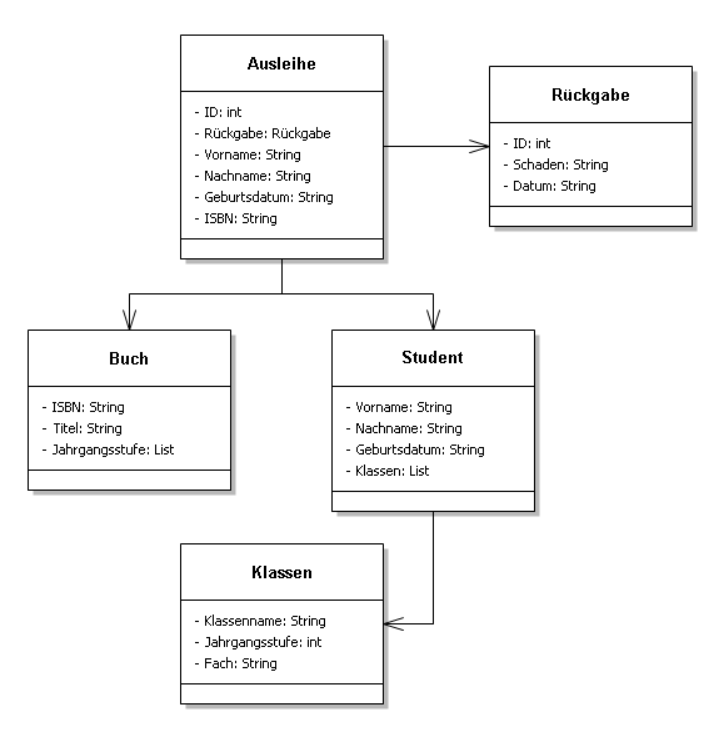
\includegraphics[width=0.55\textwidth]{figures/konzept/rueckgabe.PNG}
	\caption{Beziehungen einer Ausleihe}
	\label{fig:ausleihe}
\end{figure}
In Abbildung \ref{fig:ausleihe} sind die Beziehungen einer Ausleihe abgebildet. Eine Ausleihe benötigt dabei immer einen Studenten, welcher ausleiht, und ein Buch, welches ausgeliehen wird. Das Buch ist eindeutig definiert durch die entsprechende ISBN. Sowohl der Student, als auch das Buch werden in der Ausleihe referenziert. Eindeutig definiert ist jede Ausleihe durch einen numerischen Identifikator. Zusätzlich referenziert jede Ausleihe auf eine Rückgabe. Bei der Erstellung der Ausleihe ist diese immer leer. Erst wenn das entsprechende Buch des Studenten zurückgegeben wird, findet die Referenzierung statt. Falls das Buch Beschädigungen aufweist, werden diese ebenfalls in die Rückgabe eingetragen. Die Rückgabe ist auch durch einen numerischen Identifikator definiert.

\subsection{Benutzeroberflächen}
Sämtliche Benutzeroberflächen in LibOrg sind mittels Qt erstellt worden. Dabei beginnt das Programm derzeit immer mit einer leeren Startseite (es ist denkbar, dass in der nächsten Version der Software über die Konfiguration festgelegt wird, welches Element nach dem Starten angezeigt wird). Wählt der Benutzer in den oberen Menüleisten eine gewünschte Funktion aus, wird das entsprechende GUI angezeigt. Für die Standardfunktionen Bücher ausleihen/zurückgeben, Schüler bearbeiten und Bücher bearbeiten sind dies einfache Tabellen wie in Abbildung \ref{fig:tabelle} für das Beispiel 'Buch' zu sehen ist.
\begin{figure}[H]
	\centering
	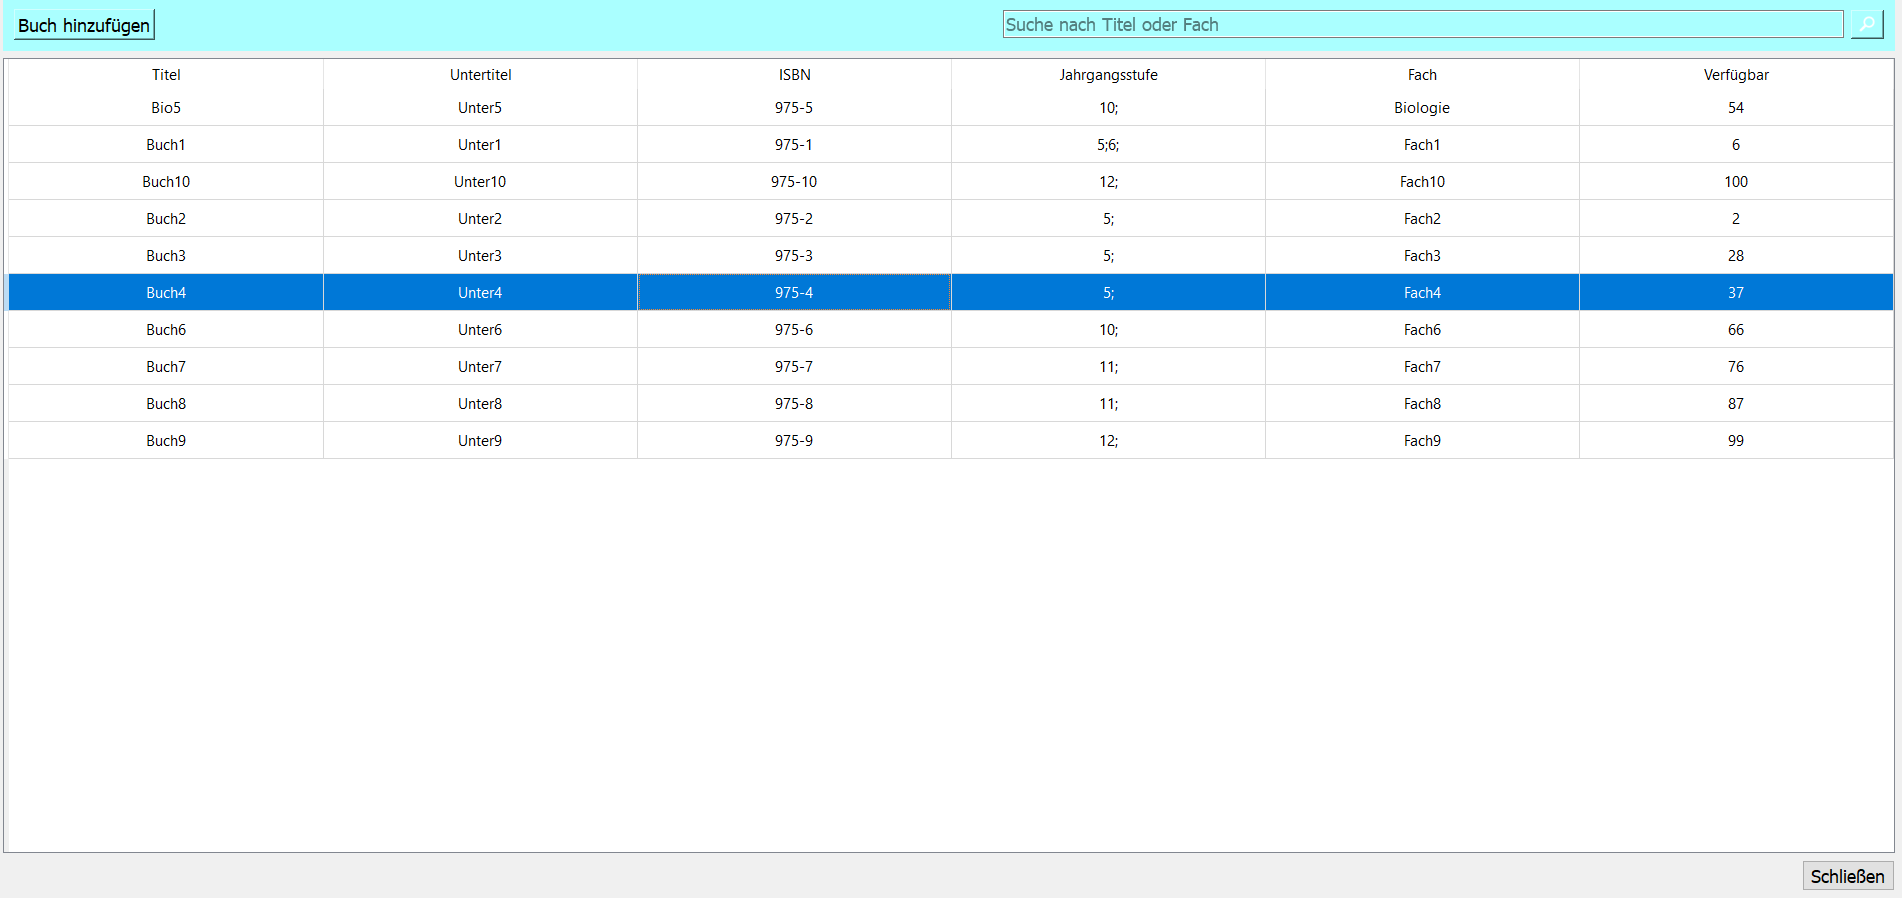
\includegraphics[width=1\textwidth]{figures/konzept/tabelle.PNG}
	\caption{Tabelle zum Anzeigen von Büchern}
	\label{fig:tabelle}
\end{figure}
Um einen Schüler oder ein Buch zu bearbeiten bzw. anzulegen, werden entsprechende Eingabemasken angezeigt, welche passende Eingabemöglichkeiten bieten (siehe Abbildung \ref{fig:maske}).
\begin{figure}[H]
	\centering
	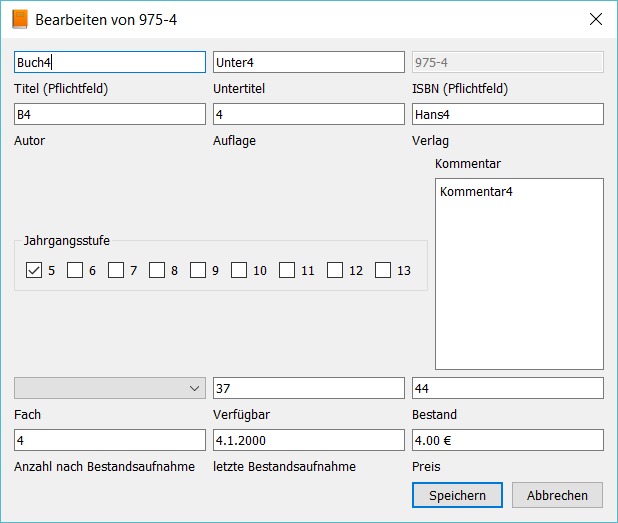
\includegraphics[width=0.60\textwidth]{figures/konzept/maske.PNG}
	\caption{Eingabemasken zum Bearbeiten eines Buches}
	\label{fig:maske}
\end{figure}
Für sonstige Aufgaben wie das Ändern der Einstellungen oder das Managen aller Benutzerkonten werden weitere passende Benutzeroberflächen angeboten.

\subsection{Plausibilisierung und Validierung}
Der Benutzer hat in LibOrg die Möglichkeit eigene Schüler und Bücher per passende Eingabemasken zu erstellen (siehe Abbildung \ref{fig:maske}). Bei der Erstellung dieser Objekte, was stattfindet sobald der Benutzer seine Angaben speichert, werden die Eingaben des Nutzers validiert. Hier wird zum Beispiel überprüft, ob ein Name oder eine ISBN (die Primary keys in der Datenbank) vorhanden sind. Für manche Einträge gibt es auch bereits fertige Eingabemasken, welche nur eine Eingabe in der vorgegebenen Form erlauben, beispielsweise das Angeben eines Datums für die letzte Bestandsaufnahme oder ein Preis für das Buch. Auch wird verboten in manchen Felder Zahlen bzw. Buchstaben anzugeben. Ein Vor- oder Nachname kann keine Zahl beinhalten und der Bestand kann nur durch Ziffern angegeben werden. Durch in grau dargestellte Platzhalter, werden dem Benutzer für jedes Feld korrekte Beispiele für die Eingabe angezeigt, wie in Abbildung \ref{fig:grey} zusehen ist.
\begin{figure}[H]
	\centering
	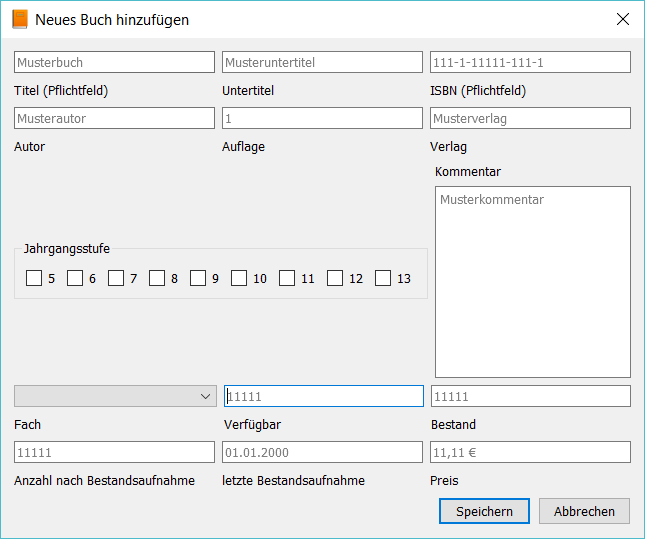
\includegraphics[width=0.60\textwidth]{figures/konzept/grey.PNG}
	\caption{Graue Platzhalter in der Eingabemaske}
	\label{fig:grey}
\end{figure}
Bei sensiblen Operation wie das Löschen eines Schülers oder eines Buches, wird der Benutzer mittels Messagebox nochmal um sein Einverständnis gefragt, damit eine versehentliche Benutzung ausgeschlossen werden kann (siehe Abbildung \ref{fig:messagebox}).
\begin{figure}[H]
	\centering
	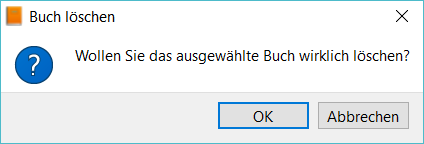
\includegraphics[width=0.30\textwidth]{figures/konzept/messagebox.PNG}
	\caption{Messagebox zur Bestätigung einer Operation.}
	\label{fig:messagebox}
\end{figure}

\subsection{Ausnahme- und Fehlerhandling}
Sämtliche Fehlerfälle welche durch das falsche Bedienen der Software ausgelöst werden können, werden von LibOrg abgefangen. Dabei wird dem Benutzer immer mitgeteilt, dass die geplante Aktion nicht möglich ist. Ein Beispiel hierfür wäre, wenn der Benutzer ein Buch löschen will, welches noch ausgeliehen ist. Dies würde intern zu einer Inkonsistenz der Datenbank führen, da eine Ausleihe das Buch entsprechend referenziert und somit das Buch nicht gelöscht werden darf. Dabei wird dem Benutzer durch eine MessageBox angezeigt, dass dies nicht möglich ist (siehe Abbildung \ref{fig:error}).
\begin{figure}[H]
	\centering
	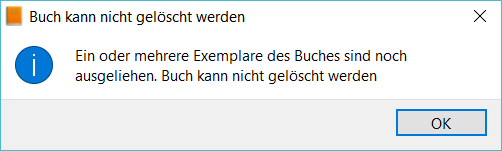
\includegraphics[width=0.40\textwidth]{figures/konzept/error.PNG}
	\caption{Messagebox zum Hinweisen des Benutzers}
	\label{fig:error}
\end{figure}
Ein Spezialfall bildet der Import von Schülern über Excel-Dateien. Da die benötigten Informationen über mehrere Excel-Dateien verteilt sind, müssen die einzelnen Schüler anhand der Namen in den einzelnen Dateien zusammengefügt werden. Hier kann es zu möglichen Fehlerfällen kommen. Zum Beispiel können die Namen der Schüler nicht genau übereinstimmen aufgrund von exotischen Namensgebungen. Auch könnte der Schüler in einer Datei existieren und in der anderen allerdings keinen Eintrag haben, dies führt ebenfalls zu einem Fehler. Nach dem Abschluss des Imports werden alle aufgetretene Fehler in einem Fenster angezeigt, wie in Abbildung \ref{fig:import} zu sehen ist. Daraufhin hat der Benutzer die Möglichkeit die Fehler über die gegebenen Standardfunktionen per Hand zu beheben.
\begin{figure}[H]
	\centering
	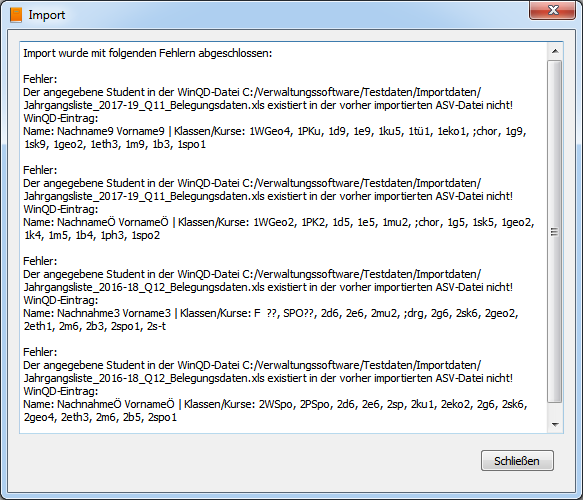
\includegraphics[width=0.60\textwidth]{figures/konzept/import.PNG}
	\caption{Fehlerausgabe nach abgeschlossenem Import.}
	\label{fig:import}
\end{figure}
Falls Daten von dem Benutzer fälschlicherweise gelöscht oder geändert werden, legt das System sicherheitshalber bei Start und beim Beenden des Programms ein Backup der aktuellen Datenbank ab. Dadurch ist es möglich jederzeit zu einem alten Stand der Datenbank zurückzukehren.

\subsection{Testbarkeit}
In LibOrg wurden sämtliche Benutzeroberflächen und die Logik dahinter 'per Hand' getestet. Hierbei wurden Excel-Listen über alle gewünschten Funktionalitäten der einzelnen Features angelegt, welche durchgegangen worden sind. \\
Per Unit-Tests wurde die komplette Datenbank-API getestet. Dies hat nicht nur den Grund, dass die komplette Anwendung auf der korrekten Funktionalität dieser API fußt, sondern auch, dass falls später die Datenbank noch erweitert wird, die Funktionalität der bisherigen API weiterhin bestätigt werden kann und dass die Änderung keine Auswirkungen auf den unveränderten Code hat (Regressionstest).
